% Created 2025-06-04 Mi 17:14
% Intended LaTeX compiler: xelatex
\documentclass[11pt]{article}
\usepackage{graphicx}
\usepackage{grffile}
\usepackage{longtable}
\usepackage{wrapfig}
\usepackage{rotating}
\usepackage[normalem]{ulem}
\usepackage{amsmath}
\usepackage{textcomp}
\usepackage{amssymb}
\usepackage{capt-of}
\usepackage{hyperref}
\usepackage{mathspec}
\usepackage{xunicode}
\usepackage[no-sscript]{xltxtra}
\author{Sebastian Meisel}
\date{\textit{<Mi,  4. Jun. 2025>>}}
\title{IPv6 prefix delegation using systemd-networkd}
\hypersetup{
	pdfauthor={Sebastian Meisel},
	pdftitle={IPv6 prefix delegation using systemd-networkd},
	pdfkeywords={},
	pdfsubject={},
	pdfcreator={Emacs 29.4 (Org mode 9.6.15)},
	pdflang={English}}

\newenvironment{menu}{}{}

\begin{document}

\maketitle

\begin{center}
	
\includegraphics[width=.65\linewidth]{img/Ostseepinguin.png}
\end{center}


\begin{menu}
	\href{NetworkNamespace.DE.html}{🇩🇪 DE}
	\begin{itemize}
		\item > \href{index.html}{Home}
	\end{itemize}

	\noindent\rule{\textwidth}{0.5pt}
	\begin{center}
		
\includegraphics[width=.65\linewidth]{img/Mastodon.png}
	\end{center} \url{https://emacs.ch/@SebasTEAan}

	📧 \href{mailto:sebastian.meisel+ostseepinguin@gmail.com}{sebastian.meisel at gmail.com}
\end{menu}

\section*{Introduction}
\label{sec:orgb6dc759}

Recently my \texttt{ISP} (Internet Service Provider) finally provided me with modern \texttt{IPv6}. I at least got an \texttt{/60} prefix, which allows me to do subnetting, with up to 16 subnets, as the network identifier in \texttt{IPv6} has \texttt{64 bits}. So far so good. But I soon realized, that my prefix changes frequently, just as the \texttt{IPv4} prefix. That however is a problem. I do have two VLANs, beside my default network, that need their own \texttt{GUA} (Global Unicast Address) prefix. So whenever my prefix changes I would need to change my VLAN configurations and my routes. That's not feasible.


Gladly there is an solution to that problem: IPv6 Prefix delegation (\texttt{PD}).

\subsection*{Set up}
\label{sec:orgeab173b}

This is how my network currently looks:

ATTR\textsubscript{HTML}: :width 100\% :alt Left: The Internet (as a cloud) is connected to a home router via fiber. From there an Ethernet connection is drawn to a switch, which is connected to a Raspberry Pi, that acts as a router. Above the switch is connected to a Wireless AP, that provides Wifi to various mobile devices in the VLAN "WLAN", which is colored light orange. Beneath a desktop PC is connected to the switch, which is in the VLAN "Office", colored in light purple.
\begin{center}
	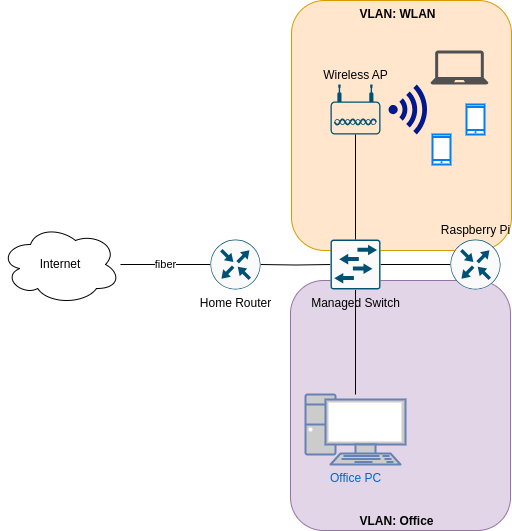
\includegraphics[width=.65\linewidth]{img/IPv6Network.png}
\end{center}



\subsection*{Configuring the WAN-interface}
\label{sec:org9a50c01}

\texttt{/etc/systemd/network/10-{}-{}eth0.network}
\begin{lstlisting}[breaklines=true,language=bash,showspaces=false,basicstyle=\small\ttfamily,keywordstyle=\color{blue},commentstyle=\color{gray},stringstyle=\color{red},numbers=left,numberstyle=\tiny,frame=tb,language=text,label= ,caption= ,captionpos=b]
[Match]
Name=eth0
Type=ether

[Network]
Description=WAN Ethernet port

DHCP=ipv6
IPv6AcceptRA=yes

VLAN=Office
VLAN=WLAN

[Address]
Address=192.168.178.254
Gateway=192.168.178.1

[DHCPv6]
PrefixDelegationHint=::/60
UseDelegatedPrefix=yes
UseAddress=no


[Route]
Gateway=192.168.178.1
\end{lstlisting}
\end{document}
